\documentclass[a4paper,12pt]{article}
\usepackage{ME_AQ_temp}
\usepackage{tabularx}

%% -------------------------------------- %%
%  - impostare il titolo della tesina in entrambe le righe 
% 
%% -------------------------------------- %%

% Definisci un titolo personalizzato

% Definizione del titolo e dell'autore
\title{Corsi Accademici di Musica Elettronica DCPL34 Conservatorio A. Casella, L'Aquila \\ \fontsize{14}{17}\bfseries\uppercase{Il Recupero Digitale dell'Archivio Sonoro di Giacinto Scelsi: Metodologie, Sfide e Prospettive Musicologiche}}
\author{Giulio Romano De Mattia \\ esame di \bfseries{Storia della Musica Elettroacustica} e \\ \bfseries{Analisi della Musica Elettroacustica}}
\date{09/06/2025}

% Sovrascrivi le impostazioni di hyperref per l'indice
\hypersetup{
    linkcolor=black, % Imposta il colore dei link dell'indice a nero
}

\begin{document}

% Pagina 1: Titolo e riassunto
\maketitle
\thispagestyle{empty}

\begin{center}
    \vspace{1cm}
    \textbf{\fontsize{12}{15}\selectfont{Sommario}}
\end{center}

La presente tesina documenta l'esperienza di laboratorio svolta presso la Fondazione Isabella Scelsi, focalizzata sul complesso progetto di recupero e digitalizzazione dell'archivio sonoro del compositore Giacinto Scelsi. Il lavoro si articola in quattro sezioni principali. La prima descrive le dimensioni, la composizione e la storia conservativa dell'archivio dei nastri magnetici, evidenziando la distinzione iniziale tra materiali di "primaria" e "secondaria" importanza e le sfide poste dalle annotazioni spesso inaffidabili del compositore. La seconda sezione approfondisce il peculiare metodo compositivo di Giacinto Scelsi, analizzando l'ambiente di registrazione domestico, il ruolo cruciale dei trascrittori nel mediare tra improvvisazione e partitura, e gli strumenti utilizzati, incluse le innovative ondioline. La terza parte è dedicata alle patologie dei nastri magnetici, illustrando problematiche come il degrado naturale, la "sticky shed syndrome" (tipica dei nastri Ampex 456), le contaminazioni biologiche, l'adesione delle spire, l'effetto pre-eco e il deterioramento delle giunture, descrivendo le procedure di trattamento adottate. Infine, la quarta sezione dettaglio la catena del trasferimento digitale: dall'architettura del sistema di digitalizzazione (basato su magnetofono Studer A800 e interfaccia Pro Tools), alla gestione delle configurazioni non standard, fino ai protocolli di post-produzione, archiviazione e documentazione fotografica, sottolineando la filosofia di preservare l'integrità documentale del materiale sonoro originale. Questo studio mira a fornire una panoramica delle metodologie, delle sfide tecniche e delle prospettive musicologiche aperte da questo significativo progetto di restauro audio.
\newpage
% Genera l'indice
\tableofcontents  

% Pagina 2: Introduzione e resto del testo
\newpage

% --- File di inclusione generato automaticamente ---
% --- Contenuto LaTeX autogenerato da introduzione.md (sezione 1) ---

\section{INTRODUZIONE}
Durante le cinquanta ore di laboratorio svolte presso la Fondazione Isabella Scelsi sotto la supervisione del \persona{M° Nicola Bernardini}{9999}{9999}, ho avuto l'opportunità di partecipare attivamente a uno dei progetti di recupero e digitalizzazione più complessi e affascinanti nel campo del restauro audio contemporaneo: il salvataggio dell'intero corpus di nastri magnetici del compositore \persona{Giacinto Scelsi}{1905}{1988}.

Il progetto, iniziato nel 2006 e tuttora in corso, rappresenta un caso paradigmatico delle sfide che il restauro audio deve affrontare quando i documenti sonori non sono semplicemente registrazioni da preservare, ma costituiscono parte integrante del processo creativo di un compositore. Come documentato da Bernardini, ''questo non sarebbe stato il classico lavoro di recupero e restauro audio''\cite{Bernardini2007recoveringgia}, poiché Scelsi utilizzava i nastri come veri e propri ''sketchpad'' compositivi, registrando improvvisazioni che sarebbero poi state trascritte in partitura da suoi collaboratori.

L'archivio conta in tutale 749 nastri magnetici, di cui 278 classificati come ''di primaria importanza'' perché contenenti le improvvisazioni originali del compositore\cite{Bernardini2012themul}. A questi si aggiungono 76 dischi in alluminio laccato recentemente scoperti, che testimoniano come Scelsi avesse iniziato a utilizzare la registrazione come strumento compositivo ancor prima dell'avvento del nastro magnetico\cite[p. 185]{Bernardini2012themul}.

La peculiarità di questo progetto risiede nella necessità di preservare non solo il contenuto musicale, ma anche quello che normalmente verrebbe considerato ''rumore'': i suoni ambientali, i click dei registratori, persino il riverbero delle stanze si sono rivelati informazioni preziose per la datazione e contestualizzazione dei materiali. Durante il laboratorio ho potuto constatare come, paradossalmente, ''il rumore elettrico aggiunto dal degrado temporale dei nastri è insignificante rispetto alla grande quantità di altro rumore'' presente nelle registrazioni originali\cite[p. 170]{Bernardini2012themul}.

Il presente lavoro documenta le tecniche e metodologie applicate in questo progetto, organizzandosi in quattro parti principali: la prima dedicata alla descrizione del patrimonio sonoro e del metodo compositivo di Scelsi; la seconda alle problematiche conservative specifiche dei nastri magnetici e alle tecniche di restauro adottate; la terza al processo di digitalizzazione e post-produzione; la quarta alle prospettive di ricerca musicologica che questo lavoro di recupero ha aperto.

L'esperienza diretta con i nastri mi ha permesso di comprendere come il restauro audio, quando applicato a documenti di processo creativo, richieda un approccio multidisciplinare che integri competenze tecniche, sensibilità musicologica e comprensione del contesto storico-culturale. In questo senso, il progetto Scelsi rappresenta un laboratorio ideale per esplorare le frontiere contemporanee del restauro audio digitale.

  % Auto-generated: include introduzione.tex
% --- Contenuto LaTeX autogenerato da sezioneI.md (sezione 2) ---

\section{L'Archivio dei Nastri}
\subsection{Dimensioni e composizione della collezione}
L'archivio sonoro di Giacinto Scelsi rappresenta uno dei corpus documentari più significativi per la comprensione della musica contemporanea del secondo Novecento. La collezione, conservata presso la Fondazione Isabella Scelsi a Roma, comprende approssimativamente 749 nastri magnetici\cite{Bernardini2007recoveringgia}, ai quali si aggiungono 76 dischi istantanei in alluminio rivestiti di lacca, recentemente scoperti insieme all'apparecchiatura di incisione utilizzata dal compositore\cite{Bernardini2012themul}.

La suddivisione archivistica operata dalla Fondazione dopo la morte del compositore nel 1988 distingue due categorie principali di materiali. I nastri di ''primaria importanza'' comprendono 278 unità contenenti improvvisazioni e materiale compositivo originale di Scelsi. I restanti nastri - di ''secondaria importanza'' - includono registrazioni di opere di altri compositori, trasmissioni radiofoniche e trasferimenti da dischi in vinile\cite[p. 184]{Bernardini2012themul}.

Questa categorizzazione, pur funzionale all'organizzazione del lavoro di digitalizzazione, si è rivelata parzialmente artificiosa. Come emerso durante le sessioni di laboratorio, numerosi nastri contengono materiali eterogenei: improvvisazioni di Scelsi alternate a registrazioni radiofoniche, frammenti compositivi originali mescolati a musiche di altri autori. Tale commistione riflette l'approccio pragmatico di Scelsi al supporto magnetico, utilizzato come ''sketchpad'' per fissare qualsiasi materiale sonoro ritenuto significativo\cite[p. 170]{Bernardini2012themul}.
\subsection{Storia dei trasferimenti e stato di conservazione}
C'è stata una primma catalogazione effettuata da \persona{Barbara Boido}{9999}{9999} subito dopo la morte di Scelsi che ad oggi è il secondo numero riportato nelle etichette dell'attuale catalogazione (NMGS<primo numero>-<secondo numero>).
Il primo tentativo sistematico di preservazione digitale risale al 1992, quando il Consiglio Direttivo della FIS ha commissionato a \persona{Frances Marie Uitti}{9999}{9999} il trasferimento dei 278 nastri - come detto precedentemente di ''primaria importanza'' - su cassette DAT (Digital Audio Tape). 

Questa operazione, pur meritoria nelle intenzioni, presentava limiti significativi. Le cassette DAT, come osservato durante il laboratorio, soffrono di un degrado ''verticale'': diversamente dai nastri analogici, dove il deterioramento è graduale, i supporti digitali diventano completamente illeggibili superata una soglia critica di degrado.

Il progetto attuale di digitalizzazione, avviato nel 2006 in collaborazione con lo Studio Coltempo di Roma e proseguito dal 2007 con l'Istituto Centrale dei Beni Sonori e Audiovisivi (ICBSA)\cite{Bernardini2012themul}, sta per concludersi dopo oltre quindici anni di lavoro. Come emerso durante le sessioni di laboratorio, il numero effettivo di nastri di primaria importanza si è rivelato significativamente superiore alle stime iniziali: dai 178 nastri identificati da Frances Marie Uitti nel 1992, si è passati a oltre 350 nastri contenenti materiale compositivo originale di Scelsi. Questa espansione del corpus è dovuta al ritrovamento di numerosi nastri di primaria importanza precedentemente classificati come secondari, confermando la natura parzialmente artificiosa della categorizzazione iniziale.

Lo stato di conservazione dei nastri presenta un quadro variegato. La maggior parte dei supporti si trova in condizioni accettabili, con un livello di rumore di fondo che, seppur presente, non compromette l'intelligibilità del contenuto sonoro. Tuttavia, circa il 2-3% della collezione presenta patologie severe che richiedono interventi specialistici prima del trasferimento digitale.  Durante le sessioni di laboratorio, è stato possibile osservare direttamente il trattamento di alcuni di questi casi problematici, richiedendo la collaborazione con i tecnici specializzati della Discoteca di Stato per l'accesso alle attrezzature specifiche come i forni per il trattamento termico e gli aspiratori per la rimozione delle muffe.
\subsection{Tipologie di supporti e loro caratteristiche tecniche}
L'analisi dei supporti magnetici utilizzati da Scelsi rivela una storia tecnologica che attraversa quattro decenni. I nastri sono tutti da 1/4 di pollice di larghezza, registrati su macchine a due piste configurate per registrazione stereofonica o, più frequentemente, mono bidirezionale.

Le marche di nastro magnetico identificate durante il laboratorio includono:

\begin{enumerate}
    \item \textbf{Scotch}: I primi nastri utilizzati da Scelsi, rappresentano i supporti magnetici americani disponibili in Europa nel dopoguerra. Questi nastri hanno generalmente mantenuto buone caratteristiche di conservazione, con occasionali problemi di adesione tra le spire.
\end{enumerate}

\begin{enumerate}
    \item \textbf{Ampex}: Particolarmente problematici risultano i nastri Ampex 456, utilizzati negli studi professionali dagli anni Sessanta. Come documentato estensivamente durante le sessioni di laboratorio, questi nastri soffrono del fenomeno della ''sticky shed syndrome'': l'idrolisi del legante poliuretanico causa il distacco dello strato magnetico dal supporto.
\end{enumerate}

\begin{enumerate}
    \item \textbf{Agfa e BASF}: Nastri di produzione tedesca che presentano la caratteristica distintiva di riportare sulla costa del nastro non solo il nome del produttore ma anche il numero di matricola della partita di produzione. Questo dettaglio si è rivelato prezioso per la datazione dei materiali.
\end{enumerate}
\subsection{\persona{Friedrich Jaecker}{9999}{9999} e l'identificazione dei contenuti}
Il musicologo Friedrich Jaecker ha compilato un catalogo a partire dai primi 350-400 nastri identificando 174 frammenti.

Nel suo catalogo del 2010, Jaecker identifica con certezza materiali riconducibili a 54 opere di Scelsi distribuiti su 57 nastri. Questo dato, confrontato con i 189 manoscritti presenti nell'archivio cartaceo e i 117 titoli pubblicati, evidenzia la complessità del rapporto tra materiale registrato e produzione compositiva finale\cite[p. 47]{Bernardiniyyyy}.

L'analisi quantitativa del catalogo Jaecker rivela pattern significativi nella descrizione dei contenuti. Le occorrenze terminologiche mostrano: ''klavier/piano'' (114 menzioni), ''ondiola'' (111), ''improvvisazione'' (110), ''gestisch/gestuale'' (15) e ''ähnlich/simile a'' (14)\cite[p. 48]{Bernardini2020Quanti}. Questa distribuzione lessicale riflette non solo la strumentazione prevalente nelle registrazioni, ma anche la natura processuale e comparativa del lavoro di identificazione.
\subsection{Metadati e informazioni periferiche}
Un aspetto critico emerso durante il laboratorio riguarda l'affidabilità delle informazioni riportate sulle scatole dei nastri. Scelsi utilizzava i contenitori come superficie di annotazione, registrando numeri di contatore, indicazioni per i trascrittori, frammenti di testo. Tuttavia, la pratica del compositore di riciclare sia nastri che contenitori rende queste annotazioni inaffidabili come fonte primaria di identificazione del contenuto.

Il database sviluppato per il progetto mantiene traccia di tutte le informazioni disponibili per ciascun nastro, includendo: numero d'ordine progressivo, produttore e tipo di nastro magnetico (come riportato sulla scatola), diametro delle flange, lunghezza misurata del nastro (in metri e piedi), materiale del nastro (acetato o poliestere), velocità di registrazione identificate, posizionamento audio (testa o coda), tipologia di registrazione, parametri tecnici del trasferimento digitale.

  % Auto-generated: include sezione1.tex
% --- Contenuto LaTeX autogenerato da sezioneII.md (sezione 3) ---

\section{Giacinto Scelsi e il suo Metodo Compositivo}
\subsection{La crisi creativa}
Il metodo compositivo sviluppato da Scelsi dopo la crisi creativa dei primi anni Cinquanta rappresenta un unicum nel panorama della musica contemporanea. Come documentato da Bernardini e Pellegrini, Scelsi sviluppò una tecnica che consisteva nel registrare lunghe improvvisazioni pianistiche, inizialmente su dischi di cera e successivamente su nastro magnetico non appena la tecnologia divenne accessibile\cite[p. 176]{Bernardini2012themul}.

Questa metodologia nasceva dalla volontà di risolvere la dicotomia tra la spontaneità zen dell'improvvisazione e il lavoro meticoloso richiesto dalla notazione occidentale.
\subsection{L'ambiente di registrazione e le condizioni tecniche}
Le registrazioni di primaria importanza furono realizzate in ambiente domestico, con un approccio che privilegiava l'immediatezza della cattura sonora rispetto alla qualità tecnica. Come emerso dall'analisi delle registrazioni durante il laboratorio, Scelsi posizionava tipicamente il registratore vicino al divano, collocava il microfono sul divano stesso e si spostava al pianoforte posto a 3-4 metri di distanza, o alle ondiole.

Questa configurazione improvvisata, produceva registrazioni di qualità mediocre dal punto di vista tecnico, ma ricche di informazioni contestuali. Il riverbero naturale degli ambienti domestici, inizialmente percepito come difetto, si è rivelato un elemento distintivo che permette di identificare il luogo di registrazione: l'appartamento di Viale Mazzini 9 presenta caratteristiche acustiche diverse da quello di Via di Sant'Teodoro 8, dove Scelsi si trasferì successivamente.
\subsection{I trascrittori e il processo di mediazione}
Il sistema di lavoro di Scelsi prevedeva la collaborazione sistematica con trascrittori specializzati, compositori che traducevano le improvvisazioni registrate in notazione convenzionale.
\persona{Vieri Tosatti}{9999}{9999} fu il primo e più longevo trascrittore, responsabile della maggior parte delle partiture orchestrali e di opere significative come i Canti del Capricorno. La collaborazione con Tosatti fu facilitata dall'acquisto da parte di Scelsi di un registratore Revox A77 identico a quello del trascrittore, permettendo l'uso di riferimenti numerici precisi basati sul contatore della macchina. \persona{Sergio Cafaro}{9999}{9999} venne coinvolto specificamente per la trascrizione delle opere pianistiche, probabilmente in parallelo al lavoro di Tosatti. \persona{Enrico Filippini}{9999}{9999} subentrò quando Tosatti, afflitto da gravi problemi di vista, non poté più continuare la collaborazione. Filippini rappresenta l'ultimo anello di questa catena di mediazione tra l'improvvisazione e la partitura finale.

L'analisi delle annotazioni sulle scatole dei nastri ha rivelato un sofisticato sistema di comunicazione tra Scelsi e i suoi trascrittori. Le scatole riportano elenchi di numeri corrispondenti alle posizioni del contatore, accompagnati da indicazioni come ''buono per tromba'', ''buono per viola'', suggerendo che le composizioni venivano concepite come mosaici di frammenti da assemblare.

Questo metodo di lavoro è confermato dalla struttura stessa delle registrazioni. L'identificazione delle ''regioni'' durante la post-produzione - segmenti delimitati dai punti di start/stop del registratore - ha rivelato che alcuni nastri contengono oltre 60 frammenti distinti, mentre altri presentano registrazioni continue di diversi minuti\cite[p. 49]{Bernardini2020Quanti}. La distribuzione statistica del numero di edits per nastro mostra una concentrazione nella fascia 7-10, con casi estremi che superano i 100 tagli, questi ultimi generalmente associati a materiali parlati piuttosto che musicali\cite[p. 49]{Bernardini2020Quanti}.
\subsection{Gli strumenti della sperimentazione}
Oltre al pianoforte, strumento principale delle prime improvvisazioni, Scelsi integrò progressivamente nel suo arsenale strumentale due ondioline, sintetizzatori analogici che permettevano l'esplorazione microtonale\cite[p. 177]{Bernardini2020Quanti}. L'analisi spettrale delle registrazioni con ondiola rivela l'uso sistematico di glissandi, battimenti e intervalli microtonali che sarebbero stati impossibili da realizzare su strumenti temperati.

I registratori utilizzati da Scelsi costituiscono essi stessi parte integrante del processo creativo. Il Revox G36, registratore a valvole ancora conservato presso la Fondazione, produce rumori meccanici caratteristici e vibrazioni delle valvole che sono entrati a far parte della ''firma sonora'' di molte registrazioni. Il successivo Revox A77, uno dei registratori a nastro più diffusi al mondo, garantiva maggiore stabilità e silenziosità operativa.

L'inventario delle macchine include anche un Tandberg, un Grundig e un Geloso, registratore italiano destinato principalmente alla dettatura. La presenza di nastri di formato ridotto compatibili solo con il Geloso conferma l'utilizzo di questa macchina, anche se l'apparecchio non è stato ritrovato nell'archivio.
\subsection{Le velocità di registrazione}
L'analisi delle velocità di registrazione utilizzate rivela scelte precise legate sia a considerazioni tecniche che estetiche. La velocità standard di 19 cm/s (7,5 pollici/secondo) predomina nelle registrazioni di lavoro. La velocità professionale di 38 cm/s (15 pollici/secondo), che garantisce maggiore risposta in frequenza e minor rumore di fondo, appare nelle registrazioni che Scelsi considerava particolarmente significative. La velocità ridotta di 9,5 cm/s (3,75 pollici/secondo) veniva impiegata per sessioni prolungate dove la durata prevaleva sulla qualità.

Particolarmente interessanti sono i nastri che presentano velocità variabili all'interno della stessa registrazione, evidenziando un uso creativo e non convenzionale del mezzo. Durante il laboratorio sono stati identificati nastri con cambi di velocità intenzionali, registrazioni sovrapposte a velocità diverse, esperimenti di feedback tra le piste.
\subsection{Le ondioline: pionierismo nella sintesi elettronica}
L'introduzione delle ondioline nell'instrumentarium di Scelsi rappresenta un momento cruciale nell'evoluzione del suo linguaggio compositivo. Questi sintetizzatori analogici precoci, inventati da \persona{Georges Jenny}{9999}{9999} nel 1941, permettevano la generazione di forme d'onda sintetiche con possibilità di controllo microtonale attraverso un ribbon controller\cite{Fourier1994}.

L'analisi spettrale delle registrazioni con ondiola, effettuata durante il laboratorio utilizzando software di analisi audio contemporanei, ha rivelato l'uso sistematico di tecniche compositive innovative: Glissandi microtonali continui impossibili da realizzare su strumenti acustici tradizionali, questi glissandi creano traiettorie sonore fluide che attraversano lo spazio delle altezze senza le costrizioni del temperamento equabile; Battimenti controllati attraverso la sovrapposizione di frequenze vicine.

  % Auto-generated: include sezione2.tex
% --- Contenuto LaTeX autogenerato da sezioneIII.md (sezione 4) ---

\section{Le Patologie dei Nastri Magnetici}
\subsection{Il degrado naturale e le correnti magnetiche}
Il degrado dei nastri magnetici è un processo inevitabile causato da molteplici fattori. La nostra realtà è attraversata da correnti magnetiche di ogni tipo che, nel tempo, causano una progressiva demagnetizzazione del segnale registrato. Questo processo trasforma gradualmente l'informazione registrata in rumore di fondo.

L'esperienza diretta con i nastri di Scelsi ha permesso di osservare come questo degrado ''naturale'' sia spesso il minore dei problemi. La qualità iniziale delle registrazioni domestiche, con il loro alto livello di rumore ambientale e distorsione, rende il deterioramento magnetico relativamente poco significativo rispetto ad altre forme di degrado fisico-chimico\cite[p. 170]{Bernardini2007recoveringgia}.
\subsection{La sindrome degli Ampex 456}
Il caso più drammatico di patologia specifica riguarda i nastri Ampex 456, considerati all'epoca della loro introduzione negli anni Sessanta come prodotti di altissima qualità per uso professionale. Durante il laboratorio ho potuto osservare direttamente le conseguenze della ''sticky shed syndrome'' che affligge questi nastri: il legante poliuretanico utilizzato nella formulazione subisce un processo di idrolisi che causa il distacco progressivo dello strato magnetico dal supporto.

Il trattamento di questi nastri richiede una procedura specializzata che ho potuto seguire in collaborazione con i tecnici della Discoteca di Stato:

\begin{enumerate}
    \item \textbf{Diagnosi preliminare}: identificazione visiva e tattile della patologia attraverso l'osservazione di residui sulla flangia e test di scorrimento manuale.
\end{enumerate}

\begin{enumerate}
    \item \textbf{Trattamento termico}: i nastri vengono collocati in forni speciali che mantengono una temperatura costante tra 49 e 53 gradi Celsius con precisione di ±0,5°C per un periodo di 4-4,5 ore.
\end{enumerate}

\begin{enumerate}
    \item \textbf{Trasferimento immediato}: il nastro deve essere digitalizzato mentre è ancora caldo, quando il legante temporaneamente consolidato dal trattamento termico mantiene la sua coesione.
\end{enumerate}

\begin{enumerate}
    \item \textbf{Singola opportunità}: come osservato durante le sessioni, questi nastri possono generalmente essere letti una sola volta dopo il trattamento. Un secondo passaggio risulta impossibile poiché il nastro lascia sul percorso della testina uno strato di ossido magnetico che appare come polvere nera e perde quasi interamente tutte le informazioni contenute in esso.
\end{enumerate}
\subsection{Muffe e contaminazioni biologiche}
Circa il 2-3% dei nastri dell'archivio Scelsi presenta contaminazioni da muffe, corrispondente a circa 10-15 nastri sul totale della collezione. La presenza di muffe è stata favorita dalle condizioni di conservazione non ottimali, particolarmente nei casi in cui i nastri erano stati conservati nelle buste di plastica che trattenevano l'umidità.

Il trattamento delle muffe, osservato durante una sessione specializzata, segue un protocollo preciso:

\begin{enumerate}
    \item \textbf{Pre-trattamento termico}: i nastri ammuffiti vengono sottoposti a un ciclo di ''cottura'' breve (circa un'ora) a temperatura moderata per essiccare la muffa e trasformarla in polvere.
\end{enumerate}

\begin{enumerate}
    \item \textbf{Aspirazione controllata}: utilizzando un aspiratore speciale con filtrazione HEPA, la muffa essiccata viene rimossa delicatamente dalle spire del nastro.
\end{enumerate}

\begin{enumerate}
    \item \textbf{Pulizia del percorso}: durante la digitalizzazione, le testine devono essere pulite frequentemente per rimuovere residui di muffa che potrebbero compromettere la lettura.
\end{enumerate}
\subsection{Adesione delle spire e problematiche meccaniche}
Un problema frequente riscontrato durante il laboratorio riguarda l'adesione delle spire, fenomeno per cui gli strati adiacenti del nastro si incollano tra loro. Questa patologia può avere diverse cause: degradazione del legante, pressione eccessiva durante lo stoccaggio, variazioni di temperatura e umidità.

Il trattamento più singolare osservato durante le sessioni riguarda l'uso del borotalco per facilitare lo scorrimento delle spire adesive. La procedura, apparentemente rudimentale ma efficace, prevede l'applicazione manuale del borotalco sulla costa del nastro mentre questo scorre lentamente. Il talco agisce come lubrificante secco, permettendo la separazione delle spire senza danneggiare lo strato magnetico. Particolarmente interessante è l'osservazione che il cigolio prodotto dalle spire adesive non è solo un sintomo del problema, ma entra effettivamente nella registrazione audio durante il trasferimento, richiedendo quindi un intervento preventivo.
\subsection{L'effetto pre-eco}
Durante l'analisi dei nastri è emerso un fenomeno particolare noto come effetto pre-eco, causato dal trasferimento magnetico tra spire adiacenti. Nei nastri conservati ''in testa'' (con l'inizio del nastro all'esterno della bobina), il segnale delle spire interne può imprimere una debole copia di sé sulle spire esterne, creando un'eco che precede il segnale principale.

Questo fenomeno, udibile in alcune registrazioni commerciali dell'epoca come il secondo album dei Led Zeppelin citato durante le sessioni, ha importanti implicazioni per la conservazione. La pratica standard prevede infatti la conservazione dei nastri ''in coda'' per minimizzare questo effetto. Tuttavia, la maggior parte dei nastri di Scelsi è stata trovata conservata ''in testa'', richiedendo una procedura di doppio riavvolgimento prima della digitalizzazione:

\begin{enumerate}
    \item Avvolgimento rapido su flangia temporanea
    \item Secondo avvolgimento su altra flangia temporanea  
    \item Trasferimento digitale con riavvolgimento finale sulla flangia originale
\end{enumerate}

Questa procedura, pur generando stress meccanico sul nastro, è necessaria per garantire la corretta conservazione post-digitalizzazione.
\subsection{Il deterioramento delle giunture}
Le giunture originali presenti sui nastri rappresentano punti di particolare fragilità. Durante il laboratorio ho potuto osservare come lo scotch utilizzato per le giunture negli anni Cinquanta-Settanta sia soggetto a un processo di degrado che lo rende fragile e privo di adesività. In diversi casi, le giunture si sono separate durante la manipolazione del nastro, richiedendo un intervento di riparazione immediato.

La procedura di rifacimento delle giunture richiede precisione e materiali appropriati:
- Rimozione completa della giuntura originale degradata
- Allineamento preciso delle estremità del nastro
- Applicazione di nuovo nastro adesivo specifico per giunture audio
- Verifica della tenuta meccanica prima del passaggio sulle testine

Fortunatamente, come notato durante le sessioni, i nastri di Scelsi presentano relativamente poche giunture rispetto ai nastri provenienti da studi di musica elettronica, dove la pratica del montaggio creava centinaia di giunture per nastro.

  % Auto-generated: include sezione3.tex
% --- Contenuto LaTeX autogenerato da sezioneIV.md (sezione 5) ---

\section{La Catena del Trasferimento Digitale}
\subsection{L'architettura del sistema di digitalizzazione}
Il processo di trasferimento digitale dei nastri di Scelsi rappresenta un equilibrio delicato tra fedeltà filologica e praticabilità tecnica. Durante le sessioni di laboratorio, ho potuto osservare e partecipare direttamente all'implementazione di una catena di digitalizzazione che, pur basandosi su standard professionali consolidati, presenta specificità dettate dalla natura peculiare del materiale trattato.

Il cuore del sistema è costituito da un magnetofono Studer A800, macchina di riferimento nell'ambito del restauro audio professionale.

La decisione di operare a 96 kHz di frequenza di campionamento e 24 bit di risoluzione rappresenta uno standard elevato ma non estremo nel campo del restauro audio\cite[p. 172]{Bernardini2007recoveringgia}. Durante le discussioni tecniche in laboratorio, Bernardini ha spiegato la logica di questa scelta:

\begin{enumerate}
    \item \textbf{96 kHz di frequenza di campionamento}: garantisce una banda passante fino a 48 kHz, ben oltre il limite dell'udibile umano ma essenziale per catturare tutti gli artefatti e i rumori ad alta frequenza che possono fornire informazioni sulla datazione e identificazione dei nastri.
\end{enumerate}

\begin{enumerate}
    \item \textbf{24 bit di risoluzione}: offre un range dinamico teorico di 144 dB, ampiamente sufficiente per catturare sia il segnale utile che il rumore di fondo senza saturazione o perdita di dettaglio nei passaggi più deboli.
\end{enumerate}

L'importanza di questi parametri diventa evidente considerando che ''proprio quando i nastri sono di minore qualità e quindi hanno la maggiore quantità di rumore, è importante fissare con precisione il rumore, tutto il rumore possibile, perché questo rumore è indicativo''. Il rumore, in questo contesto, non è un elemento da eliminare ma informazione da preservare.
\subsection{L'interfaccia Pro Tools: gestione e organizzazione}
Il segnale analogico proveniente dal magnetofono Studer A800 viene convertito in digitale attraverso un'interfaccia Digidesign 192 I/O, che rappresentava al momento dell'inizio del progetto lo standard di riferimento per le produzioni audio professionali. Questa interfaccia garantisce conversione AD/DA di alta qualità con jitter estremamente basso e stabilità di clock eccellente.

L'organizzazione delle sessioni Pro Tools segue un protocollo rigoroso sviluppato nel corso degli anni di lavoro:

\begin{enumerate}
    \item \textbf{Tracce di trasferimento grezzo}: le prime tracce contengono il trasferimento continuo del nastro a diverse velocità, quando necessario. Questo approccio permette di preservare l'integrità del trasferimento originale prima di qualsiasi intervento di editing.
\end{enumerate}

\begin{enumerate}
    \item \textbf{Tracce di layout}: due tracce mono documentano la disposizione fisica del materiale sul nastro, essenziale per comprendere la struttura delle registrazioni bidirezionali.
\end{enumerate}

\begin{enumerate}
    \item \textbf{Tracce di riproduzione}: una (mono) o due (stereo) tracce contenenti la sequenza audio completa nell'ordine identificato come corretto, con tutte le velocità di lettura appropriate applicate\cite[p. 173]{Bernardini2007recoveringgia}.
\end{enumerate}
\subsection{La gestione delle configurazioni non standard}
Un aspetto particolarmente complesso del processo riguarda la gestione dei nastri con configurazioni non standard. Durante il laboratorio ho potuto osservare diversi casi problematici:

**Nastri con velocità multiple**: alcuni nastri presentano sezioni registrate a velocità diverse all'interno della stessa bobina. La procedura prevede trasferimenti multipli dell'intero nastro a tutte le velocità possibili (9,5 cm/s, 19 cm/s, 38 cm/s), con successiva ricostruzione in post-produzione della sequenza corretta.

**Registrazioni bidirezionali**: Le modalità di registrazione variano significativamente da nastro a nastro. Le registrazioni professionali utilizzano generalmente configurazione stereo, con le due piste che procedono nello stesso verso. I nastri domestici di Scelsi presentano invece spesso configurazione mono bidirezionale, con una pista che va al dritto e l'altra al rovescio. Durante la post-produzione è quindi necessario rovesciare la seconda pista per ascoltare tutto il contenuto in sequenza.

Alcuni nastri presentano registrazioni multiple in cui Scelsi passava da una pista all'altra riportando il segnale in feedback in varie direzioni. In questi casi, come osservato durante il laboratorio, ''non si capisce veramente niente'' e si deve assumere che il primo segnale sia quello della direzione giusta, mentre gli altri sono aggiunti successivamente.
\subsection{Le eccezioni al protocollo standard}
Nel corso del progetto sono emerse situazioni che hanno richiesto deviazioni dal protocollo standard. I nastri eccezionalmente lunghi, quando digitalizzati a 96 kHz, generano file che eccedono i limiti del file system HFS+ utilizzato dai computer Mac. In questi casi specifici, documentati nel database, si è optato per una frequenza di campionamento di 48 kHz. Questa decisione, presa per soli 3-4 nastri su oltre 300, rappresenta un compromesso accettabile considerando che si tratta generalmente di registrazioni di conferenze o materiale parlato dove l'estensione in frequenza è meno critica.

Un'altra eccezione riguarda i nastri gravemente danneggiati che possono essere riprodotti una sola volta. In questi casi, contrariamente al protocollo che prevede il passaggio preliminare per la misurazione, si procede direttamente al trasferimento digitale alla velocità stimata più probabile, accettando il rischio di una lettura non ottimale piuttosto che perdere completamente il contenuto.
\subsection{Il flusso di lavoro post-trasferimento}
Una volta completato il trasferimento digitale, inizia la fase di post-produzione che, nel caso dei nastri di Scelsi, non prevede alcun intervento di restauro o pulizia del segnale. Questa scelta, apparentemente controintuitiva nel campo del restauro audio, riflette la filosofia del progetto: preservare l'integrità documentale delle registrazioni\cite[p. 188]{Bernardini2012themul}.

La post-produzione si concentra invece sull'identificazione e catalogazione dei contenuti:

\begin{enumerate}
    \item \textbf{Segmentazione in regioni}: identificazione di tutti i punti di start/stop del registratore, che delimitano le unità minime di registrazione continua.
\end{enumerate}

\begin{enumerate}
    \item \textbf{Numerazione progressiva}: assegnazione di identificatori univoci a ciascuna regione per facilitare il riferimento incrociato con il database.
\end{enumerate}

\begin{enumerate}
    \item \textbf{Annotazione testuale}: trascrizione di tutte le informazioni udibili (annunci vocali, commenti) e descrizione del contenuto musicale.
\end{enumerate}

\begin{enumerate}
    \item \textbf{Generazione di metadata}: compilazione di tutti i dati tecnici e descrittivi in formato strutturato per l'inserimento nel database.
\end{enumerate}
\subsection{Standard di archiviazione e formati}
La scelta dei formati di archiviazione riflette l'impegno verso standard aperti e duraturi. I file audio vengono salvati in formato AIFF (Audio Interchange File Format) con ordinamento dei byte big-endian, garantendo la massima compatibilità e longevità\cite[p. 174]{Bernardini2012themul}. Le sessioni Pro Tools, pur essendo in formato proprietario, vengono esportate anche in formato testo (ASCII) per preservare le informazioni di editing indipendentemente dal software specifico.

Il sistema di archiviazione prevede il salvataggio dei file digitali su un array di dischi Firewire 800 in configurazione RAID-1, più un disco aggiuntivo per il backup corrente. Al termine di ogni sessione viene eseguito un backup su disco.
\subsection{Documentazione fotografica e visiva}
La documentazione fotografica costituisce una componente essenziale del processo di archiviazione. Durante il trasferimento, vengono fotografate e scannerizzate sistematicamente tutte le scatole, i contenitori e le scritte presenti su di essi, inclusi eventuali fogli inseriti all'interno. Particolare attenzione viene dedicata alla documentazione delle giunture esistenti e delle corruzioni fisiche del nastro, con registrazione precisa della loro posizione lungo il supporto\cite[p. 172]{Bernardini2007recoveringgia}. 

Le sessioni Pro Tools vengono documentate attraverso snapshot salvati in formato TIFF, garantendo una registrazione visiva dell'organizzazione delle tracce e delle regioni identificate\cite[p. 174]{Bernardini2007recoveringgia}. Questa documentazione fotografica completa permette future verifiche e analisi senza necessità di manipolare nuovamente i nastri originali, contribuendo alla loro preservazione fisica.

  % Auto-generated: include sezione4.tex
\section{Verso il Pattern Matching}

\subsection{L'obiettivo finale del progetto}

L'obiettivo ultimo del progetto di digitalizzazione dei nastri di Scelsi, come emerso chiaramente durante le sessioni di laboratorio, va ben oltre la mera preservazione del patrimonio sonoro. Durante le nostre conversazioni, Bernardini ha spiegato come l'idea iniziale fosse quella di sviluppare una ricerca sistematica per collegare i frammenti registrati con le opere pubblicate. Questo ambizioso obiettivo richiede lo sviluppo di metodologie computazionali avanzate per stabilire corrispondenze tra le improvvisazioni e le partiture finite.

Il progetto prevede due componenti fondamentali che devono procedere in parallelo: da un lato il trasferimento digitale di tutti i nastri, dall'altro la conversione delle partiture di Scelsi in formato digitale simbolico, leggibile dalle macchine. Come sottolineato durante il laboratorio, attualmente la Fondazione dispone solo di scansioni PDF delle partiture, rendendo necessaria una digitalizzazione simbolica completa del corpus delle opere pubblicate.

\subsection{Le sfide del pattern matching musicale}

Il pattern matching tra registrazioni audio e partiture presenta sfide uniche nel caso di Scelsi. Come documentato nel catalogo Jaecker, solo 57 nastri su 273 analizzati contengono materiale identificabile con certezza, lasciando circa due terzi del materiale come "territorio inesplorato"\cite[p. 47]{bernardini_pellegrini_scelsi_2016}. Questa difficoltà di identificazione "by ear" anche da parte di esperti come Jaecker, uno dei massimi conoscitori dell'opera di Scelsi, evidenzia la necessità di approcci computazionali.

Le sfide specifiche derivano innanzitutto dalla natura improvvisativa del materiale. Le registrazioni non sono esecuzioni di partiture esistenti ma improvvisazioni che potrebbero corrispondere solo parzialmente alle opere finite. A questo si aggiunge la mediazione dei trascrittori, il cui intervento introduceva inevitabilmente un livello di trasformazione e interpretazione nel passaggio dal nastro alla partitura. 

Inoltre, la concezione compositiva a mosaico emersa dall'analisi delle annotazioni sulle scatole complica ulteriormente il quadro. I brani venivano spesso assemblati da frammenti registrati in momenti diversi, rendendo necessario non solo identificare corrispondenze puntuali, ma ricostruire l'intero processo di assemblaggio compositivo.

\subsection{Approcci metodologici proposti}

Durante le discussioni in laboratorio, Bernardini ha delineato l'approccio metodologico previsto per il pattern matching. Una volta disponibili sia i nastri digitalizzati che le partiture in formato simbolico, sarà possibile implementare algoritmi di ricerca che confrontino sistematicamente il materiale audio con le rappresentazioni simboliche delle opere.

Gli articoli scientifici di Bernardini e Pellegrini suggeriscono lo sviluppo di \citazionebreve{a software tracking application which might be able to compare moderately large corpuses of audio material along with scores in symbolic format to propose evidence of similarities to scholars and musicologists}{\cite[p. 174]{pro:scelsitapes2007}}. Questo sistema dovrebbe essere in grado di:

\begin{enumerate}
 \item Analizzare caratteristiche audio estratte dai nastri digitalizzati
 \item Confrontarle con rappresentazioni simboliche delle partiture
 \item Proporre corrispondenze probabilistiche tra frammenti e sezioni di opere
 \item Fornire strumenti di validazione per i musicologi
\end{enumerate}

\subsection{Il ruolo delle tecniche di Music Information Retrieval}

Come indicato nello studio quantitativo di Bernardini e Pellegrini, \citazionebreve{music information retrieval techniques should allow us to discover more relationships hiding behind the wall of the sheer amount of material becoming available}{\cite[p. 50]{bernardini_pellegrini_scelsi_2016}}. L'applicazione di queste tecniche al corpus di Scelsi richiede adattamenti specifici:
\begin{enumerate}

 \item Gestione della qualità variabile: le registrazioni domestiche con alto livello di rumore richiedono algoritmi robusti che possano operare anche in condizioni non ottimali.

 \item Velocità multiple: i nastri registrati a velocità diverse necessitano di tecniche che possano identificare corrispondenze indipendentemente dalla velocità di riproduzione.

 \item Timbri non convenzionali: l'uso delle ondioline introduce timbri sintetici che non hanno equivalenti diretti nelle partiture orchestrali, richiedendo approcci di matching basati su strutture melodiche e armoniche piuttosto che timbriche.
\end{enumerate}

\subsection{Implicazioni musicologiche}

Il successo del pattern matching automatico avrebbe profonde implicazioni per la comprensione del processo compositivo di Scelsi. Permetterebbe innanzitutto di mappare il percorso creativo, tracciando come i frammenti improvvisati si trasformano in opere complete attraverso il processo di trascrizione. Questo consentirebbe anche di valutare più precisamente il ruolo creativo dei trascrittori Tosatti, Cafaro e Filippini, quantificando il loro contributo nel passaggio dall'improvvisazione alla partitura finale.

Un altro aspetto fondamentale riguarda l'identificazione di materiale inedito. I frammenti che non trovassero corrispondenze con opere note potrebbero rappresentare composizioni incompiute, abbandonate o semplicemente esercizi compositivi mai destinati alla pubblicazione. Infine, l'analisi cronologica dei materiali, supportata dalle tecniche di datazione tramite rumori ambientali sviluppate durante il progetto, potrebbe rivelare pattern evolutivi nel linguaggio compositivo di Scelsi, permettendo di tracciare lo sviluppo delle sue tecniche improvvisative nel corso dei decenni.

\subsection{Stato attuale e prospettive future}

Al momento della stesura di questo articolo, il progetto di pattern matching è ancora in fase di sviluppo. La digitalizzazione dei nastri procede parallelamente alla preparazione delle partiture in formato simbolico. Come osservato da Bernardini e Pellegrini, "this paper will work as an 'appetizer' to stimulate further quantity-related research in the archive".

Le prospettive future includono non solo lo sviluppo degli strumenti computazionali, ma anche la creazione di un'infrastruttura che permetta ai ricercatori di accedere e analizzare i risultati. Il sistema dovrà bilanciare l'automazione con la necessità di validazione umana, riconoscendo che l'interpretazione finale del significato musicologico delle corrispondenze trovate rimarrà sempre compito degli studiosi.

Il progetto di pattern matching rappresenta quindi non solo una sfida tecnica, ma un'opportunità unica per penetrare nel laboratorio creativo di uno dei compositori più enigmatici del Novecento, utilizzando la tecnologia contemporanea per decifrare un processo compositivo che ha deliberatamente sfidato le convenzioni della sua epoca.
  
Il progetto di recupero e digitalizzazione dell'archivio sonoro di Giacinto Scelsi, condotto presso la Fondazione Isabella Scelsi sotto la supervisione del M° Nicola Bernardini, rappresenta un'impresa di notevole complessità e importanza nel campo del restauro audio e della musicologia contemporanea. L'esperienza diretta con i 749 nastri magnetici e i 76 dischi in alluminio laccato ha permesso di comprendere a fondo non solo le sfide tecniche legate alla conservazione di supporti fragili e spesso degradati, ma anche le peculiarità di un processo creativo unico, in cui la registrazione era parte integrante della composizione stessa.

L'analisi dell'archivio ha rivelato la necessità di un approccio multidisciplinare che superasse la semplice distinzione tra nastri di "primaria" e "secondaria" importanza, data la frequente commistione di materiali. La comprensione del metodo compositivo di Scelsi, basato sull'improvvisazione registrata e sulla successiva mediazione dei trascrittori (Tosatti, Cafaro, Filippini), è stata arricchita dallo studio delle condizioni di registrazione domestica, dall'analisi degli strumenti (incluse le ondioline) e delle velocità di registrazione variabili, che testimoniano un uso sperimentale e non convenzionale del mezzo.

Le patologie riscontrate sui nastri – dalla "sticky shed syndrome" alle muffe, dall'adesione delle spire all'effetto pre-eco – hanno richiesto l'applicazione di protocolli di restauro specifici, spesso condotti in collaborazione con istituzioni specializzate come la Discoteca di Stato. Questi interventi, sebbene mirati alla stabilizzazione fisica dei supporti, sono stati guidati dalla filosofia di preservare l'integrità documentale del materiale, inclusi i "rumori" contestuali che si sono rivelati preziosi per la datazione e la comprensione.

La catena di trasferimento digitale, implementata con standard professionali (Studer A800, Pro Tools a 96kHz/24bit), è stata adattata per gestire le configurazioni non standard dei nastri di Scelsi, come le velocità multiple e le registrazioni bidirezionali. La scelta di non intervenire con restauri invasivi sul segnale audio, ma di concentrarsi sulla catalogazione meticolosa dei contenuti e sulla documentazione fotografica, riflette l'obiettivo primario del progetto: rendere accessibile ai ricercatori un corpus sonoro il più fedele possibile all'originale, completo di tutte le sue "imperfezioni" significanti.

Questo lavoro di recupero non è solo un atto di conservazione, ma apre nuove prospettive per la ricerca musicologica. La disponibilità dell'archivio digitalizzato permetterà studi approfonditi sul processo creativo di Scelsi, sulla relazione tra improvvisazione e partitura, sul ruolo dei trascrittori e sull'evoluzione del suo linguaggio. L'esperienza condotta dimostra come il restauro audio, applicato a documenti di processo creativo, diventi esso stesso uno strumento di indagine musicologica, capace di illuminare aspetti inediti dell'opera di uno dei compositori più enigmatici del Novecento e di esplorare le frontiere del restauro audio digitale.  
\appendix
\section{Catalogazione dei DAT}
\begin{figure}[H]
    \centering
    \includegraphics[width=.8\textwidth]{docs/img/box_of_boxes_of_dats-20141125.jpg}
    \caption{DAT.}
    %\label{app:figureExtra} % Etichetta per riferirsi all'appendice
\end{figure}
\begin{figure}[H]
    \centering
    \includegraphics[width=.8\textwidth]{docs/img/elenco_Uitti.jpg}
    \caption{Elenco della Uitti.}
\end{figure}

\begin{figure}[H]
    \centering
    \includegraphics[width=.9\textwidth]{docs/img/elenco_dati_Boido-Uitti.jpg}
    \caption{Elenco dei dati di catalogazione.}
\end{figure}

\section{Ondiola}
\begin{figure}[H]
    \centering
    \includegraphics[width=.9\textwidth]{docs/ondiola-doc001-01.pdf}
    \includegraphics[width=.9\textwidth]{docs/ondiola-doc001-02.pdf}
    \caption{Ondiola.}
\end{figure}

\begin{figure}[H]
    \centering
    \includegraphics[width=.8\textwidth]{docs/ondiola-doc002.pdf}
    \caption{Elenco della sintesi degli strumenti e dei settings.}
\end{figure}

\section{Registratori a nastro rinvenuti nella Fondazione Scelsi}

\begin{figure}[H]
    \centering
    \includegraphics[width=.8\textwidth]{docs/img/DSCN0037.JPG}
    \caption{Revox.}
\end{figure}

\begin{figure}[H]
    \centering
    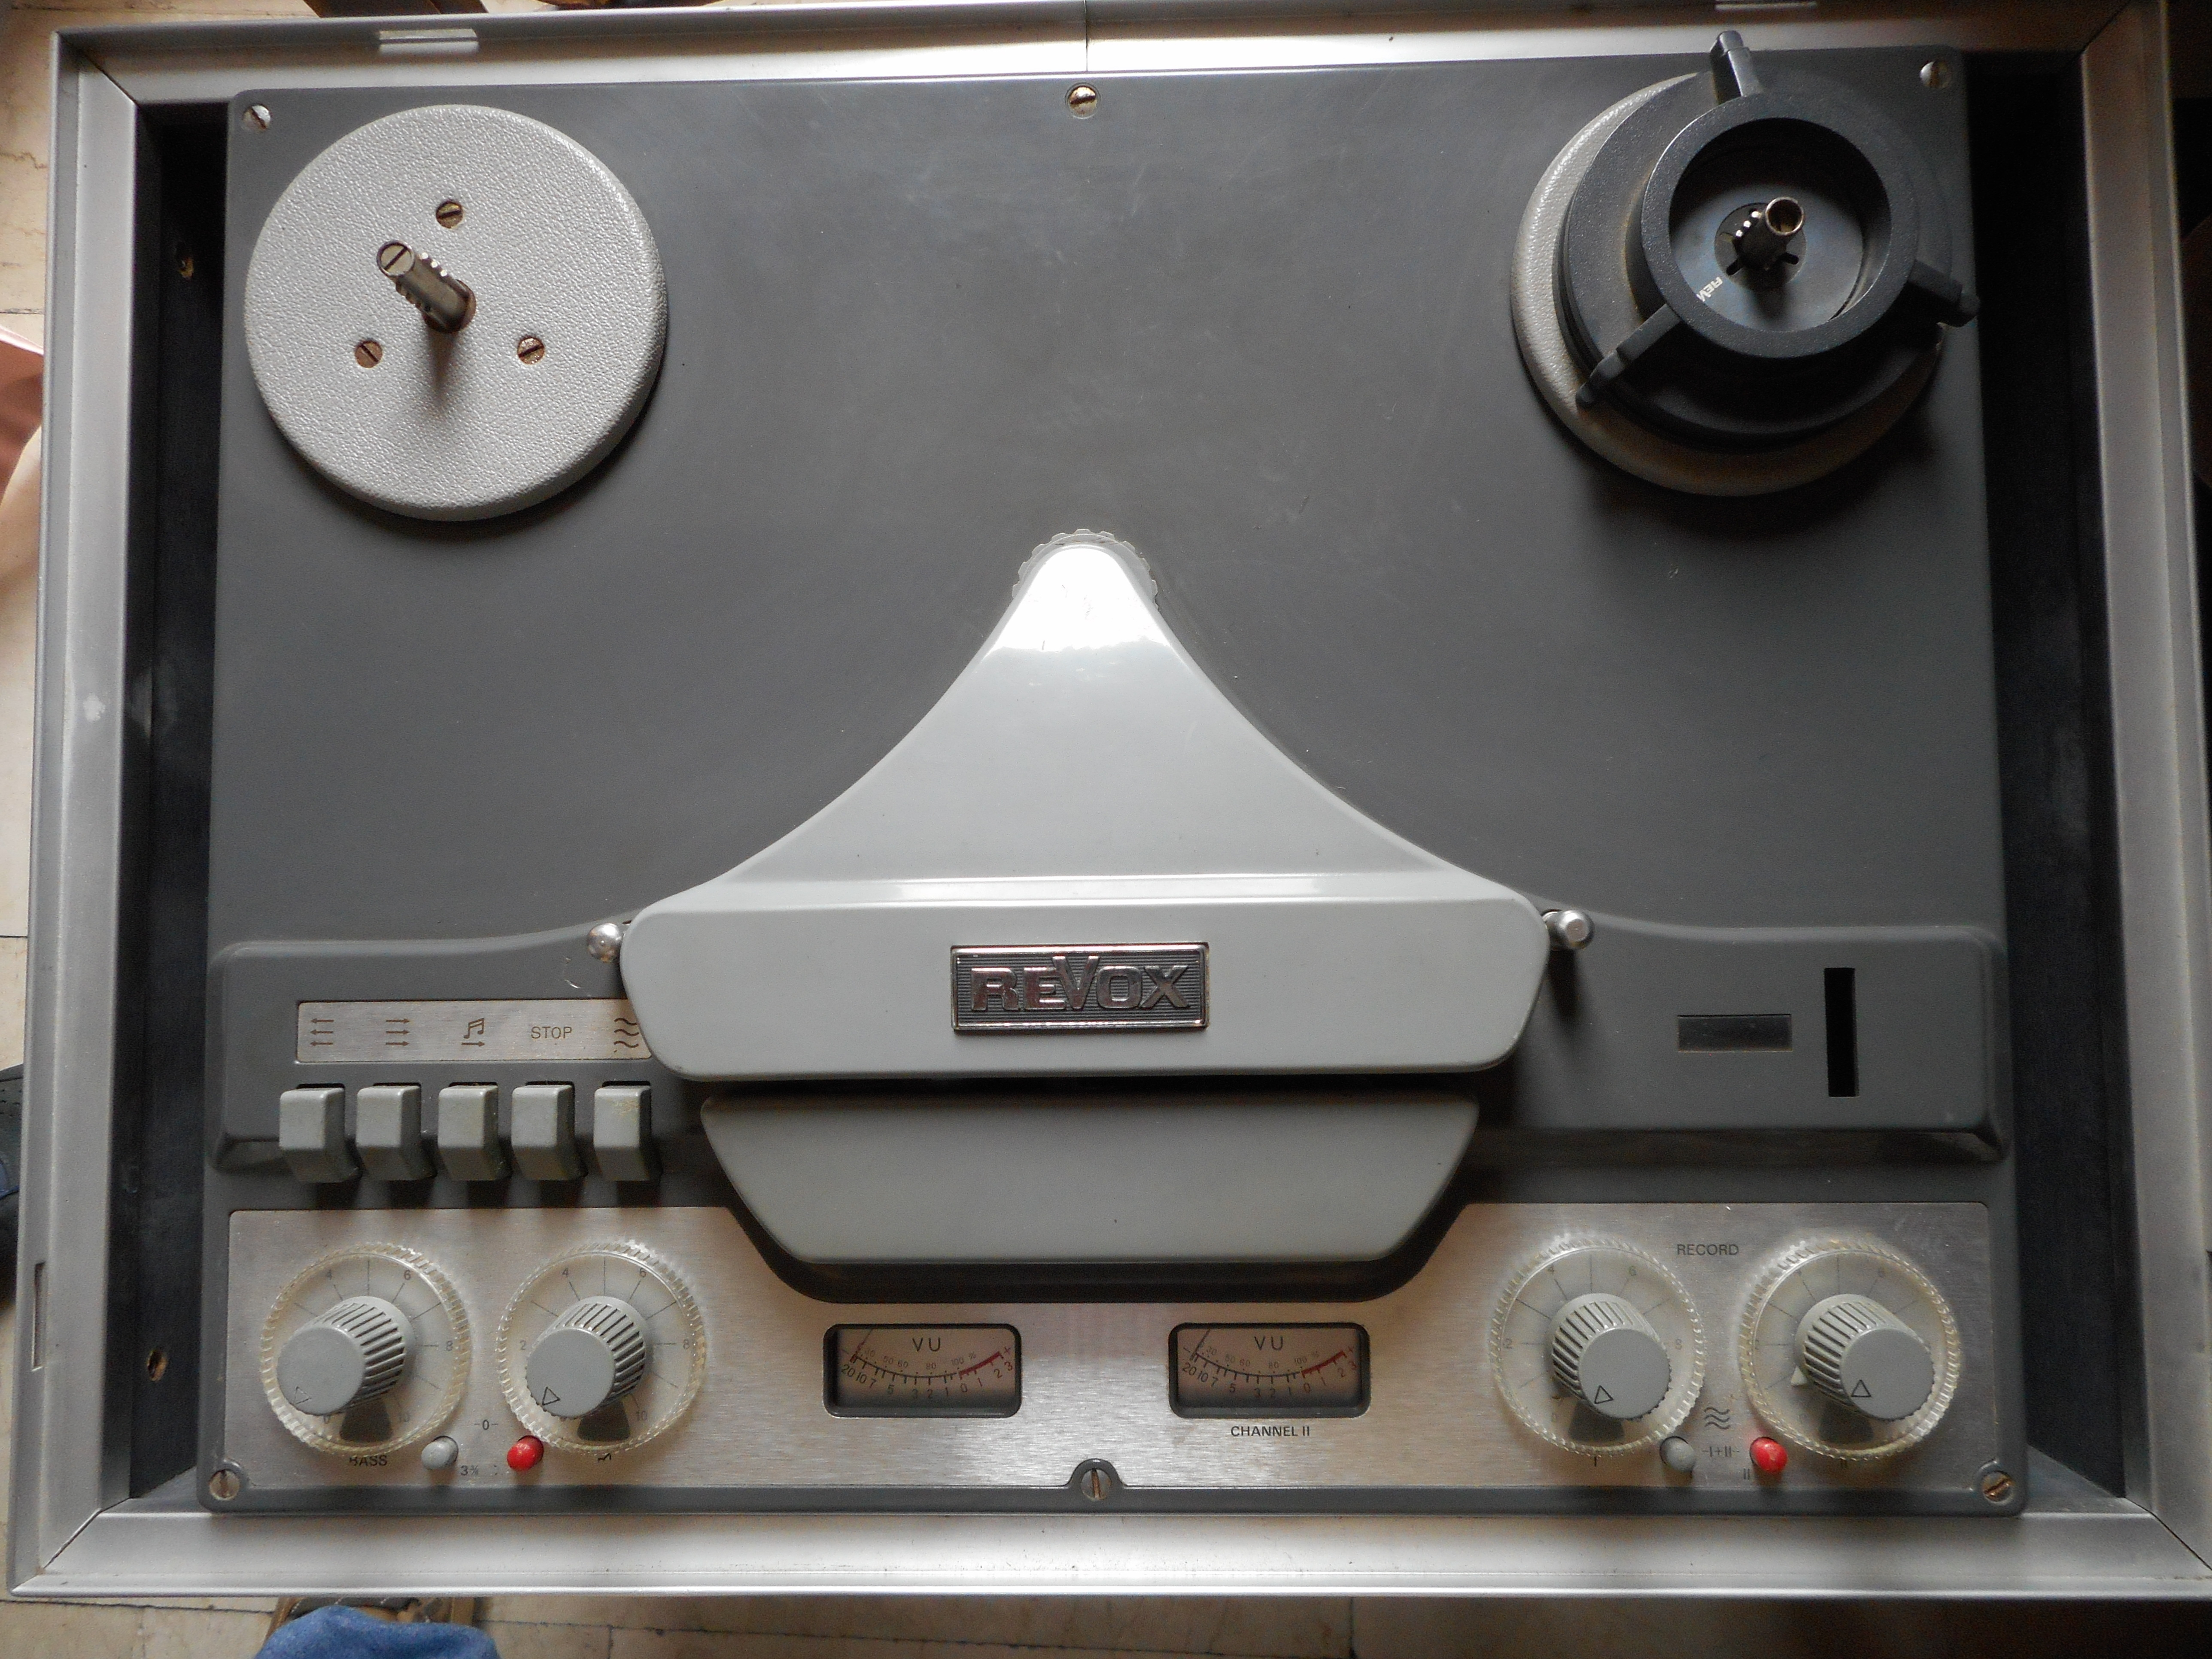
\includegraphics[width=.8\textwidth]{docs/img/DSCN0046.JPG}
    \caption{Revox.}
\end{figure}

\begin{figure}[H]
    \centering
    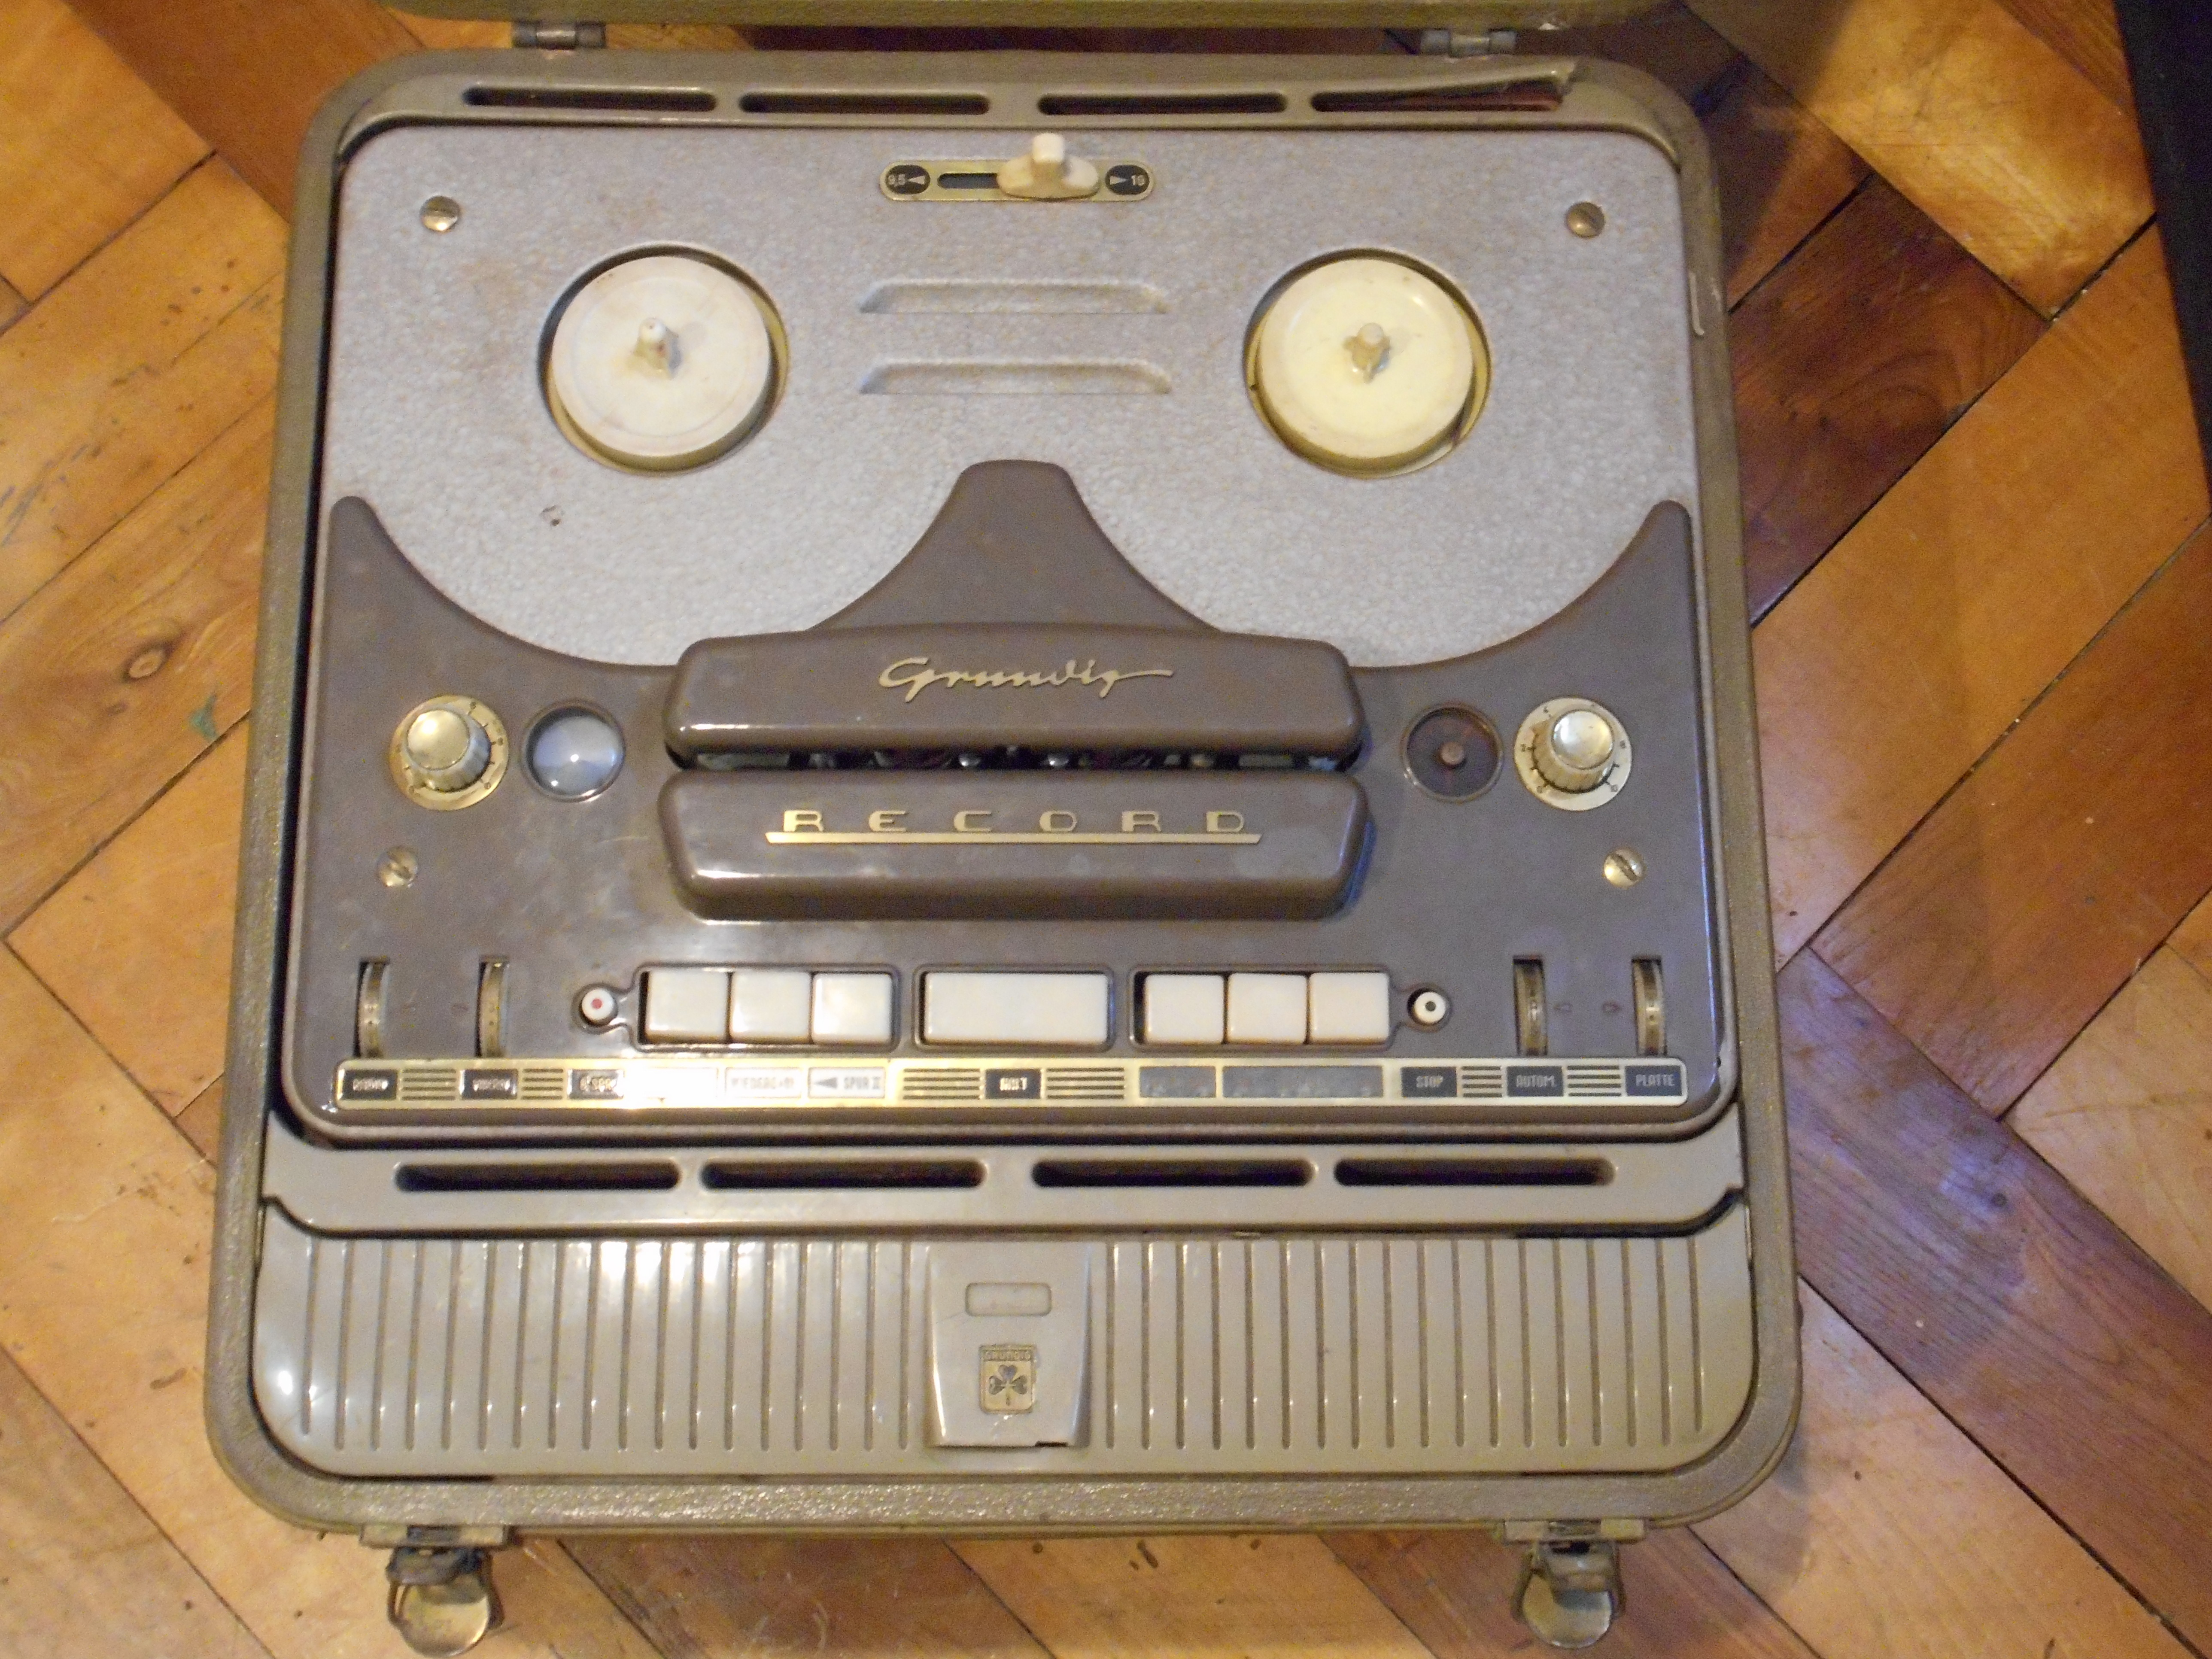
\includegraphics[width=.8\textwidth]{docs/img/DSCN0054.JPG}
    \caption{Grundig.}
\end{figure}

\begin{figure}[H]
    \centering
    \includegraphics[width=.8\textwidth]{docs/img/DSCN0060.JPG}
    \caption{Tandberg.}
\end{figure}

\begin{figure}[H]
    \centering
    \includegraphics[width=.8\textwidth]{docs/img/graveur-IMG_0877.JPG}
    \caption{Incisore di dischi Graveur.}
\end{figure}

\begin{figure}[H]
    \centering
    \includegraphics[width=.8\textwidth]{docs/img/graveur-IMG_0876.JPG}
    \caption{Incisore di dischi Graveur.}
\end{figure}



% Aggiungi la bibliografia
\newpage % ---- Inizia una nuova pagina prima della bibliografia
\bibliographystyle{plain}
\bibliography{bibliography_generated}

\end{document}